% mnras_template.tex 
%
% LaTeX template for creating an MNRAS paper
%
% v3.0 released 14 May 2015
% (version numbers match those of mnras.cls)
%
% Copyright (C) Royal Astronomical Society 2015
% Authors:
% Keith T. Smith (Royal Astronomical Society)

% Change log
%
% v3.0 May 2015
%    Renamed to match the new package name
%    Version number matches mnras.cls
%    A few minor tweaks to wording
% v1.0 September 2013
%    Beta testing only - never publicly released
%    First version: a simple (ish) template for creating an MNRAS paper

%%%%%%%%%%%%%%%%%%%%%%%%%%%%%%%%%%%%%%%%%%%%%%%%%%
% Basic setup. Most papers should leave these options alone.
\documentclass[fleqn,usenatbib]{mnras}

% MNRAS is set in Times font. If you don't have this installed (most LaTeX
% installations will be fine) or prefer the old Computer Modern fonts, comment
% out the following line
\usepackage{newtxtext,newtxmath}
% Depending on your LaTeX fonts installation, you might get better results with one of these:
%\usepackage{mathptmx}
%\usepackage{txfonts}

% Use vector fonts, so it zooms properly in on-screen viewing software
% Don't change these lines unless you know what you are doing
\usepackage[T1]{fontenc}

% Allow "Thomas van Noord" and "Simon de Laguarde" and alike to be sorted by "N" and "L" etc. in the bibliography.
% Write the name in the bibliography as "\VAN{Noord}{Van}{van} Noord, Thomas"
\DeclareRobustCommand{\VAN}[3]{#2}
\let\VANthebibliography\thebibliography
\def\thebibliography{\DeclareRobustCommand{\VAN}[3]{##3}\VANthebibliography}


%%%%% AUTHORS - PLACE YOUR OWN PACKAGES HERE %%%%%


% Only include extra packages if you really need them. Common packages are:
\usepackage{graphicx}	% Including figure files
\usepackage{amsmath}	% Advanced maths commands

%%%%%%%%%%%%%%%%%%%%%%%%%%%%%%%%%%%%%%%%%%%%%%%%%%

%%%%% AUTHORS - PLACE YOUR OWN COMMANDS HERE %%%%%

% Please keep new commands to a minimum, and use \newcommand not \def to avoid
% overwriting existing commands. Example:
\newcommand{\gcm}{g\,cm$^{-3}$}	% g per cm-cubed
\newcommand\todo[1]{\textcolor{red}{\textbf{#1}}}
\newcommand{\kepler}{{\it Kepler}}
\newcommand{\corot}{{\it CoRoT}}
\newcommand{\tess}{{\it TESS}}
\newcommand{\plato}{{\it PLATO}}
\newcommand{\gaia}{{\it Gaia}}
\newcommand{\JWST}{{\it JWST}}
\newcommand{\ngts}{{NGTS}}
\newcommand{\wasp}{{WASP}}
\newcommand{\coralie}{{CORALIE}}
\newcommand{\harps}{{HARPS}}
\newcommand{\feros}{{FEROS}}
\newcommand{\gpe}{{GP-EBOP}}
\newcommand{\LSO}{La Silla Observatory}
\newcommand{\PAR}{Paranal Observatory}
\newcommand{\etop}{\emph{top}}
\newcommand{\emid}{\emph{middle}}
\newcommand{\ebot}{\emph{bottom}}
\newcommand{\eleft}{\emph{left}}
\newcommand{\eright}{\emph{right}}
\newcommand{\eTop}{\emph{Top}}
\newcommand{\eMid}{\emph{Middle}}
\newcommand{\eBot}{\emph{Bottom}}
\newcommand{\eLeft}{\emph{Left}}
\newcommand{\eRight}{\emph{Right}}
\newcommand{\btgc}[1]{\textcolor{blue}{[BTG: #1]}}
\newcommand{\jsj}[1]{\textcolor{blue}{[JSJ: #1]}}
\newcommand{\pete}[1]{\textcolor{blue}{#1}}
\newcommand{\rgw}[1]{\textcolor{red}{#1}}
% UNITS
\newcommand{\kms}{km\,s$^{-1}$}
\newcommand{\ms}{m\,s$^{-1}$}
\newcommand{\mss}{\mbox{m\,s$^{-2}$}}
\newcommand{\masy}{mas\,yr$^{-1}$}
\newcommand{\mpl}{\mbox{$M_{p}$}}
\newcommand{\rpl}{\mbox{$R_{p}$}}
\newcommand{\mstar}{\mbox{$M_{\star}$}}
\newcommand{\rstar}{\mbox{$R_{\star}$}}
\newcommand{\mjup}{\mbox{$M_{\rm Jup}$}}
\newcommand{\rjup}{\mbox{$R_{\rm Jup}$}}
\newcommand{\msun}{\mbox{$M_{\odot}$}}
\newcommand{\rsun}{\mbox{$R_{\odot}$}}
\newcommand{\rearth}{R$_{\oplus}$}
\newcommand{\mearth}{M$_{\oplus}$}
\newcommand{\gccc}{g\,cm$^{-3}$}
\newcommand{\ergscm}{erg\,s$^{-1}$cm$^{-2}$}
\newcommand{\vsini}{$v\sin{i}$}
\newcommand{\teff}{$T_{\rm eff}$}
\newcommand{\feh}{\mbox{$\rm [Fe/H]$}}
\newcommand{\logg}{$\log g$}
\newcommand{\tc}{$T_C$}
\newcommand{\rprs}{\mbox{R$_{p}/$R$_{s}$}}
\newcommand{\vdag}{(v)^\dagger}
\newcommand\latex{La\TeX}

% Catalogue data
\newcommand{\Tstarra}{$12^{\rm h}40^{'}08.78^{"}$}
\newcommand{\Tstardec}{$-44^{\circ}18^{'}43.48^{"}$}

\newcommand{\TGAIAGmag}{$9.9103 \pm 0.0004$}
\newcommand{\TGAIAPMRA}{$-3.72 \pm 0.097$}
\newcommand{\TGAIAPMDec}{$-13.68 \pm 0.12$}
%\newcommand{\TGAIAPMplx}{$5.223 \pm  0.048$}
%\newcommand{\TGAIAPMplx}{$5.2231 \pm  0.0482$}
\newcommand{\TGAIAplx}{$9.38 \pm 0.06$}

\newcommand{\TESSTmag}{$9.4628 \pm 0.006$}
\newcommand{\TESSTmagshort}{\mbox{$11.62$}}
\newcommand{\APASSBmag}{$10.675 \pm 0.024$}
\newcommand{\APASSVmag}{$10.09 \pm 0.03$}

\newcommand{\MASSJ}{$8.903 \pm 0.037 $ }
\newcommand{\MASSH}{$8.594 \pm 0.063$ }
\newcommand{\MASSK}{$8.502 \pm 0.024$ }

% Host Properties
%\newcommand{\Tstardensity}{\mbox{$1.496 \pm 0.085$}}
%\newcommand{\Tstarage}{\mbox{$3.9 \pm 1.6$}}
\newcommand{\TTeff}{ $ 5733.0 \pm 16.0 $ }
\newcommand{\Tg}{ $ 86.5 \pm 1.8 $ }
\newcommand{\Tlogg}{ $ 4.46 \pm 0.02 $ }
\newcommand{\TFeH}{ $ 0.14 \pm 0.02 $ }
\newcommand{\TMs}{ $ 0.997 \pm 0.01 $ }
\newcommand{\TRs}{ $ 1.032 \pm 0.026 $ }
\newcommand{\Ttzerozero}{ $ 1570.1^{+0.005}_{-0.004} $ }
\newcommand{\Ttzeroone}{ $ 1798.22 \pm 0.19 $ }
\newcommand{\Tsrv}{ $ 10^{+140}_{-10} $ }
\newcommand{\Tlogsrv}{ $ 2.0 \pm 3.0 $ }
\newcommand{\Tsphot}{ $ 0.008 \pm 0.01 $ }
\newcommand{\Tlogsphot}{ $ -4.8^{+1.0}_{-1.6} $ }
\newcommand{\Tphotamp}{ $ 0.0^{+0.23}_{-0.0} $ }
\newcommand{\Tphotlogamp}{ $ -5.6 \pm 4.1 $ }
\newcommand{\Terrcontrzero}{ $ 0.67^{+0.6}_{-0.47} $ }
\newcommand{\Tlogerrcontrzero}{ $ -0.4 \pm 0.9 $ }
\newcommand{\Terrcontrone}{ $ 4.7e-06 \pm 1.9e-06 $ }
\newcommand{\Tlogerrcontrone}{ $ -12.28 \pm 0.41 $ }
\newcommand{\Terrcontr}{ $ 0.27^{+0.86}_{-0.22} $ }
\newcommand{\Tlogerrcontr}{ $ -1.3^{+1.4}_{-1.7} $ }
\newcommand{\Tmeanzero}{ $ -0.4 \pm 2.3 $ }
\newcommand{\Tmeanone}{ $ -0.0^{+0.001}_{-0.002} $ }
\newcommand{\Tmean}{ $ 7287.0 \pm 1.3 $ }
\newcommand{\Tampzero}{ $ 50.0 \pm 19.0 $ }
\newcommand{\Tlogampzero}{ $ 3.9 \pm 0.37 $ }
\newcommand{\Tampone}{ $ 6.5e-05^{+3.2e-05}_{-2e-05} $ }
\newcommand{\Tlogampone}{ $ -9.65 \pm 0.38 $ }
\newcommand{\Tamp}{ $ 18.0^{+17.0}_{-11.0} $ }
\newcommand{\Tlogamp}{ $ 2.91^{+0.66}_{-0.86} $ }
\newcommand{\TQzero}{ $ 1.0^{+2.0}_{-0.9} $ }
\newcommand{\TlogQzero}{ $ -0.0^{+1.1}_{-2.5} $ }
\newcommand{\TdeltaQ}{ $ 0.2^{+2.8}_{-0.2} $ }
\newcommand{\TlogdeltaQ}{ $ -1.9^{+2.9}_{-9.0} $ }
\newcommand{\TPzero}{ $ 2.541^{+0.0}_{-0.001} $ }
\newcommand{\TPone}{ $ 6.745^{+0.009}_{-0.008} $ }
\newcommand{\TKzero}{ $ 2.16 \pm 0.28 $ }
\newcommand{\TlogKzero}{ $ 0.77 \pm 0.13 $ }
\newcommand{\TKone}{ $ 3.56 \pm 0.39 $ }
\newcommand{\TlogKone}{ $ 1.27 \pm 0.11 $ }
\newcommand{\Tecczero}{ $ 0.09^{+0.09}_{-0.066} $ }
\newcommand{\Teccone}{ $ 0.046^{+0.069}_{-0.035} $ }
\newcommand{\Tomegazero}{ $ -0.3 \pm 1.0 $ }
\newcommand{\Tomegaone}{ $ 0.0 \pm 1.8 $ }
\newcommand{\TMpzero}{ $ 4.56 \pm 0.6 $ }
\newcommand{\TMpone}{ $ 10.5 \pm 1.2 $ }
\newcommand{\Trorzero}{ $ 0.0195 \pm 0.0014 $ }
\newcommand{\Tlogrorzero}{ $ -3.936 \pm 0.071 $ }
\newcommand{\Trorone}{ $ 0.0001^{+0.0029}_{-0.0001} $ }
\newcommand{\Tlogrorone}{ $ -9.0 \pm 3.2 $ }
\newcommand{\Trplzero}{ $ 2.06 \pm 0.14 $ }
\newcommand{\Trplone}{ $ 0.01^{+0.3}_{-0.01} $ }
\newcommand{\Tbzero}{ $ 0.45 \pm 0.2 $ }
\newcommand{\Tbone}{ $ 0.5^{+0.36}_{-0.35} $ }
\newcommand{\Trhopgcmthreezero}{ $ 2.85^{+0.76}_{-0.62} $ }
\newcommand{\Trhopgcmthreeone}{ $ 0^{+440000000000}_{-0} $ }
\newcommand{\Tperiod}{ $ 22.5^{+3.8}_{-1.6} $ }
\newcommand{\Tlogperiod}{ $ 3.11^{+0.16}_{-0.08} $ }
\newcommand{\Tmix}{ $ 0.06^{+0.17}_{-0.04} $ }
\newcommand{\TphotSzero}{ $ 0.012 \pm 0.003 $ }
\newcommand{\Tphotwzero}{ $ 3.62^{+0.46}_{-0.41} $ }
\newcommand{\Tphotmean}{ $ 0.011^{+0.034}_{-0.038} $ }
\newcommand{\TaRszero}{ $ 7.828 \pm 0.026 $ }
\newcommand{\TaRsone}{ $ 15.009 \pm 0.051 $ }
\newcommand{\Tsmazero}{ $ 0.038 \pm 0.001 $ }
\newcommand{\Tsmaone}{ $ 0.072 \pm 0.002 $ }
\newcommand{\TSinzero}{ $ 1000000 \pm 13000 $ }
\newcommand{\TSinone}{ $ 272000 \pm 3600 $ }
\newcommand{\TTsurfpzero}{ $ 1370.4^{+4.4}_{-4.6} $ }
\newcommand{\TTsurfpone}{ $ 989.7 \pm 3.3 $ }
\newcommand{\Ttdurzero}{ $ 0.099^{+0.006}_{-0.007} $ }
\newcommand{\Ttdurone}{ $ 0.127^{+0.019}_{-0.049} $ }

%\newcommand{\TdelTshort}{\mbox{$390.0082$}}
%\newcommand{\TdelT}{\mbox{$390.0082 \pm 0.0032$}}

\newcommand{\TSindexlogerrcontr}{ $ -5.12 \pm 0.16 $ }
\newcommand{\TSindexerrcontr}{ $ 0.006 \pm 0.001 $ }
\newcommand{\TSindexmean}{ $ 0.1 \pm 9.9 $ }
\newcommand{\TSindexlogamp}{ $ -9.72^{+0.5}_{-0.42} $ }
\newcommand{\TSindexamp}{ $ 6e-05^{+3.9e-05}_{-2.1e-05} $ }
\newcommand{\TSindexlogQzero}{ $ 0.2 \pm 1.1 $ }
\newcommand{\TSindexQzero}{ $ 1.2^{+2.0}_{-0.9} $ }
\newcommand{\TSindexlogdeltaQ}{ $ -4.9^{+5.2}_{-7.5} $ }
\newcommand{\TSindexdeltaQ}{ $ 0.0^{+1.3}_{-0.0} $ }
\newcommand{\TSindexlogperiod}{ $ 3.67^{+0.15}_{-0.48} $ }
\newcommand{\TSindexperiod}{ $ 39.0 \pm 11.0 $ }
\newcommand{\TSindexmix}{ $ 0.49 \pm 0.4 $ }

% \newcommand{\Tplanetmass}{\mbox{$0.344 \pm _{0.073}^{0.092}$}}
% \newcommand{\Tplanetradius}{\mbox{$0.817 \pm _{0.032}^{0.028}$}} 
% \newcommand{\Teq}{\mbox{$435 \pm _{32}^{34}$}}
% \newcommand{\Tpgrav}{\mbox{$14.1 \pm _{3.4}^{5.3}$}}
% \newcommand{\TpH}{\mbox{$141 \pm _{51}^{74}$}}
% \newcommand{\Tpa}{\mbox{$0.2010 \pm _{0.0022}^{0.0021}$}}
% \newcommand{\Tpincl}{\mbox{$89.16 \pm _{0.29}^{0.20}$}}
% \newcommand{\Tpden}{\mbox{$0.78 \pm _{0.17}^{0.21} $}} % g/cm^3

\newcommand{\TTstar}{TOI-755}
\newcommand{\TTplanet}{TOI-755.01}
\newcommand{\Tstar}{HD\,110113}
\newcommand{\Tplanet}{HD\,110113\,b}
\newcommand{\Tplanetc}{HD\,110113\,c}
\newcommand{\TGAIAid}{6133384959942131968}
\newcommand{\TICstar}{TIC-73228647}
\newcommand{\Tperiodshort}{2.5}

%%%%%%%%%%%%%%%%%%%%%%%%%%%%%%%%%%%%%%%%%%%%%%%%%%

%%%%%%%%%%%%%%%%%%% TITLE PAGE %%%%%%%%%%%%%%%%%%%

% Title of the paper, and the short title which is used in the headers.
% Keep the title short and informative.
\title[\Tplanet]{\Tplanet\,(\TTplanet)- a hot mini-Neptune transiting a Sun-like star}

% The list of authors, and the short list which is used in the headers.
% If you need two or more lines of authors, add an extra line using \newauthor
\author[H.P. Osborn et al.]{
\parbox{\textwidth}{H.P. Osborn,$^{{1},{2}}$\thanks{E-mail: hugh.osborn@space.unibe.ch},
D.J. Armstrong$^{3,4}$, % D.J.Armstrong@warwick.ac.uk
V. Adibekyan$^{5}$, % Vardan.Adibekyan@astro.up.pt
E. Delgado-Mena$^{5}$,
G. King$^{3,4}$, %
J.F. Otegi$^{6}$, %
N.C. Santos$^{5,7}$, % Nuno.Santos@astro.up.pt
}\\
% List of institutions
$^{1}$NCCR/PlanetS, Centre for Space \& Habitability, University of Bern, Bern, Switzerland\\
$^{2}$Department of Physics and Kavli Institute for Astrophysics and Space Research, MIT, 70 Vassar Street, Cambridge, MA 02139, USA\\
$^{3}$Centre for Exoplanets and Habitability, University of Warwick, Gibbet Hill Road, Coventry, CV4 7AL, UK\\
$^{4}$Department of Physics, University of Warwick, Gibbet Hill Road, Coventry CV4 7AL, UK \\
$^{5}$Instituto de Astrof\'isica e Ci\^encias do Espa\c{c}o, Universidade do Porto, CAUP, Rua das Estrelas, 4150-762 Porto, Portugal\\
$^{6}$Geneva Observatory, University of Geneva, Chemin des Mailettes 51, 1290 Versoix, Switzerland\\
$^{7}$Departamento de F\'isica e Astronomia, Faculdade de Ci\^{e}ncias, Universidade do Porto, Rua do Campo Alegre, 4169-007 Porto, Portugal\\
}

% These dates will be filled out by the publisher
\date{Accepted XXX. Received YYY; in original form ZZZ}

% Enter the current year, for the copyright statements etc.
\pubyear{2020}

% Don't change these lines
\begin{document}
\label{firstpage}
\pagerange{\pageref{firstpage}--\pageref{lastpage}}
\maketitle

% Abstract of the paper
\begin{abstract}
We report the discovery of \Tplanet{}(\TTplanet{}), a transiting mini-Neptune exoplanet on a 2.5-day orbit around a sunlike G-type star (\teff{}= $5730$K).
Using \tess{} photometry and \harps{} radial velocities, we find \Tplanet{} has a radius of \Trplzero{}\rearth{} and a mass of \TMpzero{} \mearth{}.
The resulting density of \Trhopgcmthreezero{}\gcm{} is significantly lower than would be expected from a pure-rock world, therefore \Tplanet{} must be a mini-Neptune with significant volatile atmosphere.
Given the high incidental flux and low surface-gravity of the planet, we find it unusual that \Tplanet{} was able to hold onto it's atmosphere over its $\sim4$Gyr lifetime.
We also find a non-transiting planet with a mass of \TMpone{} \mearth{} and a period of \TPone{}d, although a strong stellar rotation signal with period \Tperiod{}d impedes its confirmation.
\end{abstract}

% Select between one and six entries from the list of approved keywords.
% Don't make up new ones.
\begin{keywords}
planets and satellites: detection -- stars: individual: HD110113
\end{keywords}

%%%%%%%%%%%%%%%%%%%%%%%%%%%%%%%%%%%%%%%%%%%%%%%%%%

%%%%%%%%%%%%%%%%% BODY OF PAPER %%%%%%%%%%%%%%%%%%

\section{Introduction}


\section{Observations}

\subsection{TESS photometry}
\Tstar{} was observed during \tess{} sector 10 with 2-minute cadence for 22.5 days, excluding a 2.5 day gap between TESS orbits to downlink data.
The lightcurve was processed using the Pre-Search Data Conditioning (PDC) pipeline, producing precise detrended photometry with typical precision of 150ppm/hr.
This lightcurve was then searched for exoplanetary candidates with the SPOC (Science Processing Operations Centre).
Vetting identified a strong candidate with a period of 2.54, a depth of only 400ppm and a Signal to Noise Ratio (SNR) of 7.6.
It was designated TESS Object of Interest (TOI) 755.01. 

\subsection{HARPS RVs}
Over the course of two observing seasons in 2018 and 2019, a total of N high-resolution spectra were taken with the High Accuracy Radial velocity Planet Searcher on the 3.4m telescope at La Silla, Chile.
These radial velocities were taken as part of the NCORES program designed to specifically study the internal structure of hot worlds.

The HARPS spectra and derived RVs were accessed and downloaded through the DACE portal hosted at the University of Geneva \citep{2015ASPC..495....7B}.

\subsection{Ground-based Photometric Observations}
Karen ToDo

\subsection{Speckle imaging}
Howell ToDo

\section{Analysis}

\subsection{Stellar Parameters}
Stellar parameters (\teff and \logg) and [Fe/H] were derived using
a recent version of the MOOG code (Sneden 1973) and a set of plane-paralel
ATLAS9 model atmospheres (Kurucz 1993). The analysis was done in LTE. The methodology used is described 
in detail in Sousa et al. (2011) and Santos et al. (2013). The full spectroscopic analysis is 
based on the Equivalent Widths (EWs) of 233 Fe i and 34 Fe ii weak lines
by imposing ionization and excitation equilibrium. The line-list used
was taken from Sousa et al. (2008). 


\subsection{Combined RV and Photometric modelling}

\subsubsection{Treatment of Radial Velocities}
All RV indicator statistics showed clear signs of stellar variability, likely due to the presence of starspots.
To remove this stellar activity we first turned to linear decorrelation of the RV signal using RV indicators.
The FWHM and S-index showed the clearest rotational signals, so we selected these and used the decorrelation technique provided with the DACE spectroscopy python package \citep{2015ASPC..495....7B}\footnote{\url{https://dace.unige.ch/tutorials/?tutorialId=34}}.
Despite the activity indicators removing much of the stellar variability signal, the peak at \Tperiod{} remained strong in the radial velocity timeseries (see Figure \ref{fig:rv_decorr}).
After removing the rotation signal at $23.68\pm0.08$ by fitting a Keplerian, the next strongest signals were at $6.73\pm0.03d$ and $2.541\pm0.0008d$ with amplitudes of $3.88\pm0.31 ms^{-1}$ and $2.55\pm0.31$ respectively. This was followed by signals on longer periods which are most likely spurious due to rotational and observational aliases.

% (see Figure \ref{fig:LS}), therefore we chose this as the indicator with which to train a GP.
Although this linear decorrelation and Keplerian-fitted rotation period was able to reveal the planetary RV signals, stellar variability cannot in general be modelled as a Keplerian.
Instead we turned to a Gaussian process (GP) model to model the impact of rotation on the RVs.
One GP kernel well-suited to stellar rotation is to use a decay term multiplied by a mix of rotational terms corresponding to $P_{\rm rot}$ and $P_{\rm rot}/2$, which we built using \texttt{celerite} \citep{foreman2017fast}.
In order to limit the impact of the GP on the planetary RV signal, we fitted activity time series and RV timeseries simultaneously with the same GP kernel, as these should follow the same underlying variations with the exception of planetary signals.
To do this, the hyper-parameters for rotation period, decay timescale, the mix factor, and the signal quality ($Q$ \& $\delta Q$) were kept constant, while the signal amplitude \& mean were taken from three different distributions corresponding to each of S-index, FWHM and RV. 
For each time-series we also used a jitter term to model noise not included by measurement errors and to prevent GP over-fitting.
%To train the GP we used a Rotational kernel , with a fifth parameter to include excess jitter in the measurements. 
All hyper-parameters were given broad priors, although the rotation period was constrained to the value obtained from a Lomb-Scargle periodogram with a standard deviation of 40\%.
%We optimised this model and then ran a Hamiltonian Monte Carlo to produce 1200 samples from which to use as priors in our RV GP model. The resulting GP model fit is shown in figure \ref{SindexFig}.

A 2-parameter (e.g. linear) trend term was included to model potential long-term drift in the RVs.

\begin{figure}
	% To include a figure from a file named example.*
	% Allowable file formats are eps or ps if compiling using latex
	% or pdf, png, jpg if compiling using pdflatex
	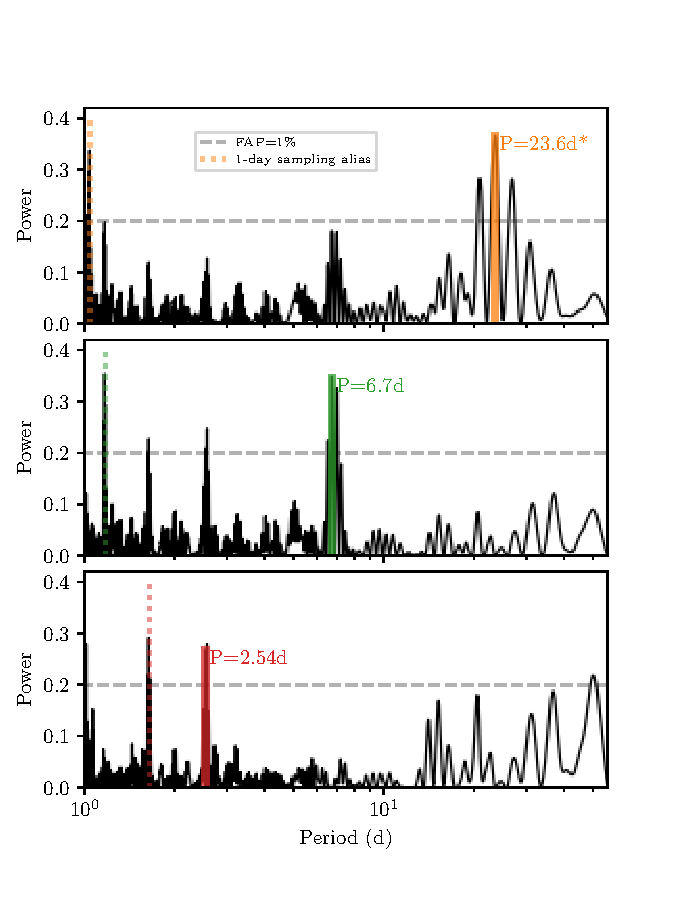
\includegraphics[width=\columnwidth]{TOI755_decorrelation_periodograms}
    \caption{Periodograms of RVs after linear decorrelation with S-index and FWHM. The upper panel shows the raw periodogram, while subsequent panels show the periodogram after the removal of the previously marked peak. The 2.54d peak is accompanied by a significant peak at the 1-day sampling alias (1.65d), but the knowledge of a 2.54d planet in the TESS photometry breaks this degeneracy.}
    \label{fig:rv_decorr}
\end{figure}
% \begin{figure}
% 	% To include a figure from a file named example.*
% 	% Allowable file formats are eps or ps if compiling using latex
% 	% or pdf, png, jpg if compiling using pdflatex
% 	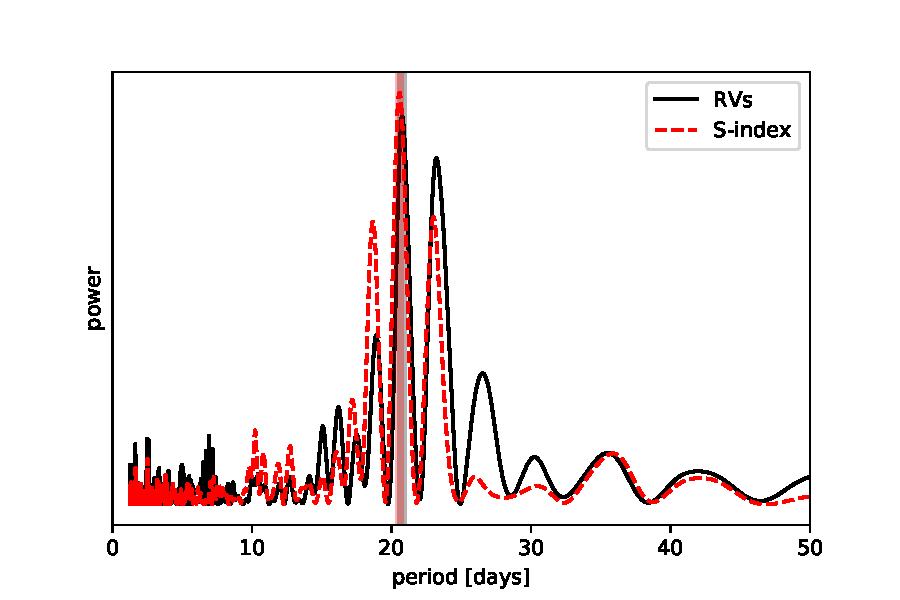
\includegraphics[width=\columnwidth]{LombScargle_755}
%     \caption{The Lomb-Scargle of both the S-index and RV. Overplotted in grey are the derived maximum signals which are in close agreement and suggest a rotation period of \TSindexperiod}
%     \label{fig:Sindex}
% \end{figure}

\onecolumn
\begin{figure}
	% To include a figure from a file named example.*
	% Allowable file formats are eps or ps if compiling using latex
	% or pdf, png, jpg if compiling using pdflatex
	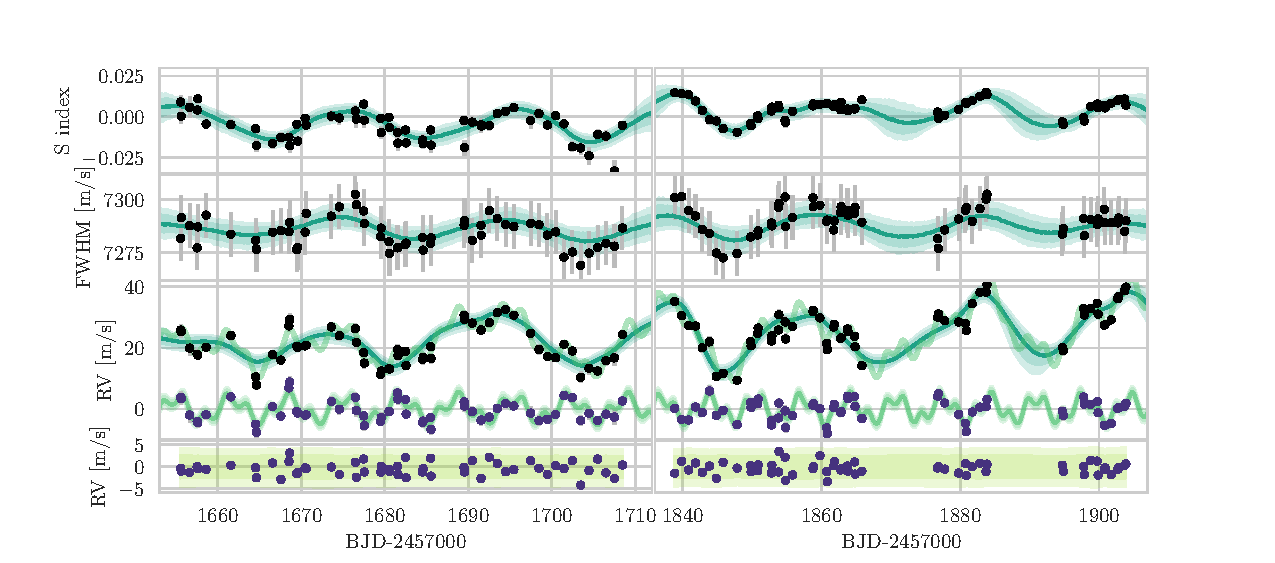
\includegraphics[width=\textwidth]{Combined_RV_plots_3_GPs.pdf}
    \caption{S-index, FWHM and RV timeseries, with GP models and 2-sigma uncertainty regions overplotted in green. Below the raw RV timeseries is the GP-removed timeseries showing the sum of the two planets models, and their uncertainties. At the very bottom the full model residuals are shown, with an RMS of only 1.50\ms{} only 0.11\ms{} above the average HARPS measurement uncertainties.}
    \label{fig:RVs}
\end{figure}
\twocolumn

\begin{figure}
	% To include a figure from a file named example.*
	% Allowable file formats are eps or ps if compiling using latex
	% or pdf, png, jpg if compiling using pdflatex
	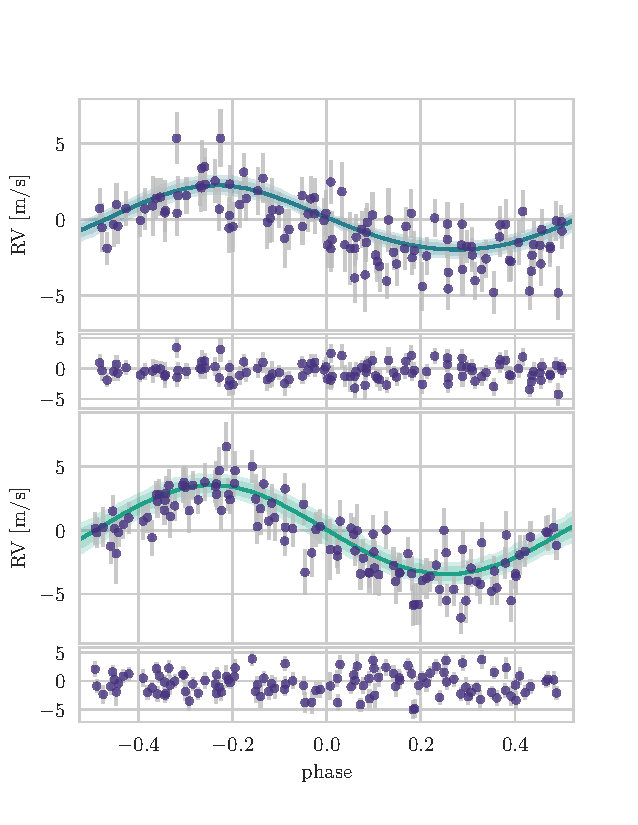
\includegraphics[width=\columnwidth]{Phase_folded_RV_plots_3_GPs}
    \caption{The phase-folded RV lightcurves for \Tplanet{} and \Tplanetc{}.}
    \label{fig:phase_fold_rvs}
\end{figure}

\subsubsection{Treatment of Photometry}
First, we normalised the \texttt{PDC\_SAP} timeseries and masked anomalous flux points from the timeseries by cutting data more than $4.2\sigma$ above both preceding and succeeding neighbours.

We initially tried to use the same \texttt{celerite} GP kernel to predict both RV and photometric time series deviations.
This proved to not be possible, likely because the effect of stellar variability on photometry is not necessarily at the same timescale as for RVs \citep{10.1111/j.1365-2966.2011.19960.x}.
Similarly, although a Lomb-Scargle periodogram of the raw TESS lightcurve does show a peak with a period around 25d, the processed \texttt{PDC\_SAP} lightcurve is flat, likely as variability on  the order of a TESS orbit ($\sim 14d$) are removed during processing.
Instead we used a separate, single-SHO kernel with quality $Q=1/\sqrt{2}$ to model the photometric stellar variability.
To produce the initial hyperparameters and priors for the combined analysis and reduce the possibility of the GPs attempting to model out the transits themselves, we first fitted this GP to the photometry with planetary transits cut. The interpolated posterior distributions from this analysis then provided the priors for the combined analysis.
A jitter term was also included to model the effect of high-frequency noise not fully encapsulated by the photon noise (e.g. stellar jitter).

We modelled the limb darkening using two approaches - one where limb darkening is fitted for for the data alone using the reparameterisation of \citet{kipping2013efficient}, and another where the theoretical limb darkening parameters for the star as generated by \citet{claret2017limb} are used as priors for the analysis.
We found the resulting distributions to be consistent, and chose to use the constrained approach in the final modelling.
Radius ratio $R_p/R_s$ was treated using the log amplitude to avoid negative values, and $R_p/R_s$ \& b were reparameterised following the \texttt{exoplanet} implementation of \citet{espinoza2018efficient}.

As ground-based photometry was unable to produce significant transit measurements, we restrict this analysis to only the \tess{} photometry and \harps{} spectroscopy.

\subsubsection{Combined Model}
We modelled full keplerian orbits for the two planets, with eccentricity priors according to the \citet{kipping2013parametrizing} beta distribution.

Monte Carlo sampling, while able to explore the parameter space around a best-fit solution, does not deal well with exploring unconstrained parameters with multiple local minima. 
This is specifically true with planetary period and epoch, especially in the case of the 6.7d planet which does not appear to have corresponding transit events. 
Therefore, in order to allow our model to explore a single solution, we included normal priors on period and $t_0$ using the values and uncertainties from the TOI catalogue in the case of the $2.54$d planet, and from the RV periodogram in the case of the $6.7$d planet.

The combined model, built using \textsf{exoplanet} \citep{exoplanet} package, was sampled using the No-U Turn Sampler (NUTS) in the Hamiltonian Monte Carlo \texttt{PyMC} back-end \citep{exoplanet:pymc3} to produce 3600 independent samples (after 500 steps tune-in).

The results from the combined model are shown in table \ref{table:datatable}, with the \harps{} RV timeseries and best-fit models shown in figure \ref{fig:RVs}, phase-folded RVs and model shown in figure \ref{fig:phase_fold_rvs}, and \tess{} photometry and best-fit light curves shown in figure \ref{fig:photometry}.

\onecolumn
\begin{figure*}
	% To include a figure from a file named example.*
	% Allowable file formats are eps or ps if compiling using latex
	% or pdf, png, jpg if compiling using pdflatex
	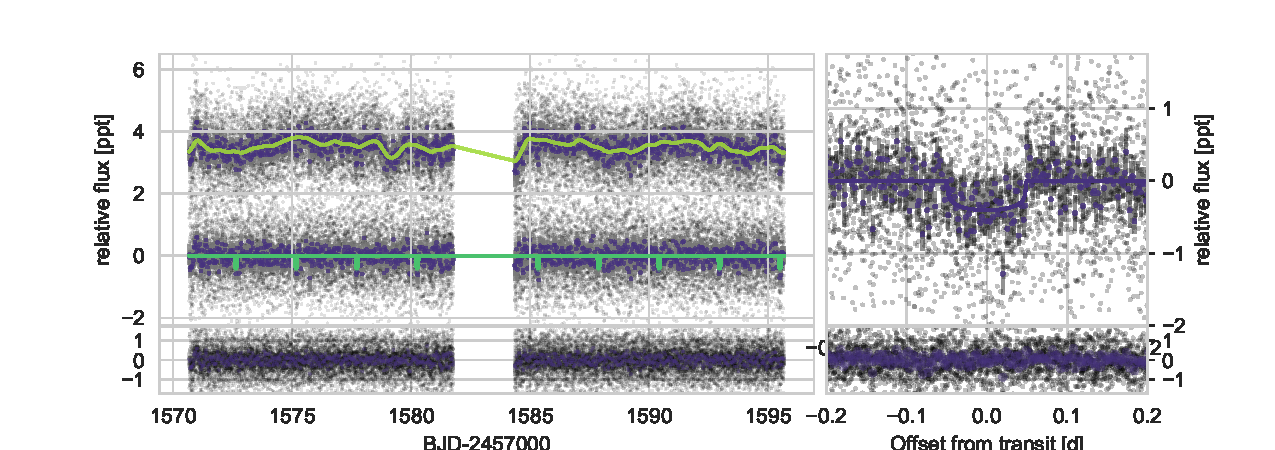
\includegraphics[width=\textwidth]{Combined_phot_plot_3_GPs}
    \caption{\tess{} photometry, where black dots represent individual 2-minute cadence data and dark circles (with errorbars) represent 30-minute bins. Upper left: \tess{} \texttt{PDC\_SAP} time series with best-fit GP model (both offset by 3.5ppt), and GP-subtracted lightcurve with the best-fit transit model over-plotted (no offset). Lower left: residuals, with both GP model and transit models subtracted from the lightcurve. Upper right: phase-folded lightcurve of \Tplanet{} zoomed to the transit. Lower right: phase-folded residuals. }
    \label{fig:photometry}
\end{figure*}
\twocolumn

As a cross-reference, these models were


\subsection{Other potential planet candidates}
Both Kepler and TESS have shown that multi-planet systems of small planets in resonant orbits close to their star are common \citep{?}.
Therefore, it is worth exploring whether signals of other candidate planets are present in either the TESS photometry or the RV time series.

We ran the \texttt{transit least squares} algorithm \citep{heller} on the model-subtracted lightcurve and found...

Present in the RV periodogram (and, interestingly, not in the activity periodograms) is a relatively strong peak at around 7 days.
The best-fitting combined two-planet model (limiting planet c to non-transiting solutions) produces an outer planet with a potential mass of $TBD$ on a period of $TBD$.
The parameters for the planet b remain within errorbars 
Although \texttt{exoplanet} does not allow the computation of Bayesian evidence, we can use the log likelihoods of the best-fitting 1-planet model with the best-fitting 2-planet model to compute the difference in Bayesian Inference Criterium ($\Delta{\rm BIC}$.
This value is $TBD$ in favour of a TBD.
However, such a peak also corresponds to exactly $P_{\rm rot}/3$, and may be an alias of the rotation period.

The corresponding \texttt{TLS} periodogram shows no peak at this period suggesting that, if it is due to an outer planet, the planet is either grazing or non-transiting.
Such a candidate planet would likely also be near an $8/3$ resonance with \Tplanet, and therefore could be characterised using TTVs. 
However, the low-SNR nature of this planet means that no significant TTVs are currently detectable.
\Tplanet will be re-observed by \tess during Sector 37\footnote{\url{https://heasarc.gsfc.nasa.gov/cgi-bin/tess/webtess/wtv.py?Entry=73228647}}

\section{Methods, Observations, Simulations etc.}

Normally the next section describes the techniques the authors used.
It is frequently split into subsections, such as Section~\ref{sec:maths} below.
%
%\begin{table*}[t]
%    \centering
%    \caption{Catalogued, measured and derived properties of \Tstar\ and \Tplanet. 
%    % Pete - I commented out the following cos its not needed I think
%    %Asymmetric errors are reported in brackets and correspond to the difference between the median and the 16$^{th}$ (lower value) and 84$^{th}$ (upper value) percentile. Asymmetric errors which differed by a factor of 2 are reported in quadrature as symmetric uncertainties with $\pm$.
%    }
%    \begin{tabular}{cc|cc}
%    \hline
%    \hline
%    \multicolumn{2}{l}{Catalogue data} & \multicolumn{2}{l}{Model parameters}     \\
%    \hline
%%Gaia Source ID & \TGAIAid        & $T_0$ (BJD-TDB) & \TfitTO  \\
%TIC ID & \TICstar        & $T_0$ (BJD-TDB) & \Ttzerozero  \\
%R.A.  &  \Tstarra      & $P$ (d) &  \TP \\
%decl.  & \Tstardec     & $b$  & \Tb \\
%G & \TGAIAGmag         & $u_{\rm TESS}(0)$ & \Tuzero \\
%%BP & \TGAIABPmag                 & $b$          & \Tfitb \\
%%RP & \TGAIARPmag                &  $h_{1,\rm \tess}$  & \TfithItess  \\
%pmRA (\masy)   & \TGAIAPMRA  & $u_{\rm TESS}(1)$ & \Tuone \\
%pmDec (\masy)  & \TGAIAPMDec &  $K_\star$ (\kms) & \TlogK \\
%Parallax ($\rm mas$) & \TGAIAplx 
%\tess\ (T)   & \TESSTmag 
%% APASS9 (B) & \APASSBmag 
%% APASS9 (V) & \APASSVmag & $\sqrt{e}\sin \omega$ & \Tfitfs  \\
%% APASS9 (g') & \APASSgmag & $\sqrt{e}\cos \omega$& \Tfitfc  \\
%% APASS9 (r') & \APASSrmag &  $\gamma$ (\kms)& \TfitV \\ 
%% APASS9 (i') &\APASSimag & $\Delta \gamma_{\rm FEROS}$ (\kms)& \TfitHF\\
%\cline{3-4}
%2MASS (J)  & \MASSJ  &  \multicolumn{2}{l}{Derived planet properties} \\
%\cline{3-4}
%2MASS (H)  & \MASSH  & \mpl\ (\mjup) & \Tplanetmass \\
%2MASS (K$_{\rm s}$)& \MASSK &  \rpl\ (\rjup) &  \Tplanetradius  \\
%\cline{1-2}
%\multicolumn{2}{l|}{Stellar parameters} &  $a\,(\rm au)$ & \Tpa \\  
%\cline{1-2}
%\teff\ (K) &  \Tteff & e & \Tfite   \\
%\feh\ ($\rm dex$) &  \TFeH &  $\omega$ (deg) & \Tfitw \\  
%$\log g_\star$ ($\rm dex$) &  \Tlogg &  $i$ (deg) & \Tpincl  \\
%%\vsini\ (\kms) & \Trotation  &  $T_{\rm dur}$ (hr) & \Tfitdur \\
%\mstar\ (\msun) &  \TMs  & $g_p$ (\mss)& \Tpgrav\\
%\rstar\ (\rsun) & \TRs  & $T_{\rm eq}$ $(\rm K)$ & \Teq  \\
%%$\rho_\star$\ ($\rho_{\sun}$) & \Tstardensity & $\rho_{p}$\ (g\,cm$^{-3}$) & \Tpden  \\
%%Age $(\rm Gyr)$ & \Tstarage & $H_p$ (km)& \TpH \\
%\hline
%    \end{tabular}
%    \label{table:datatable}
%\end{table*}

% \begin{figure*}
% \makebox[\textwidth][c]{
%  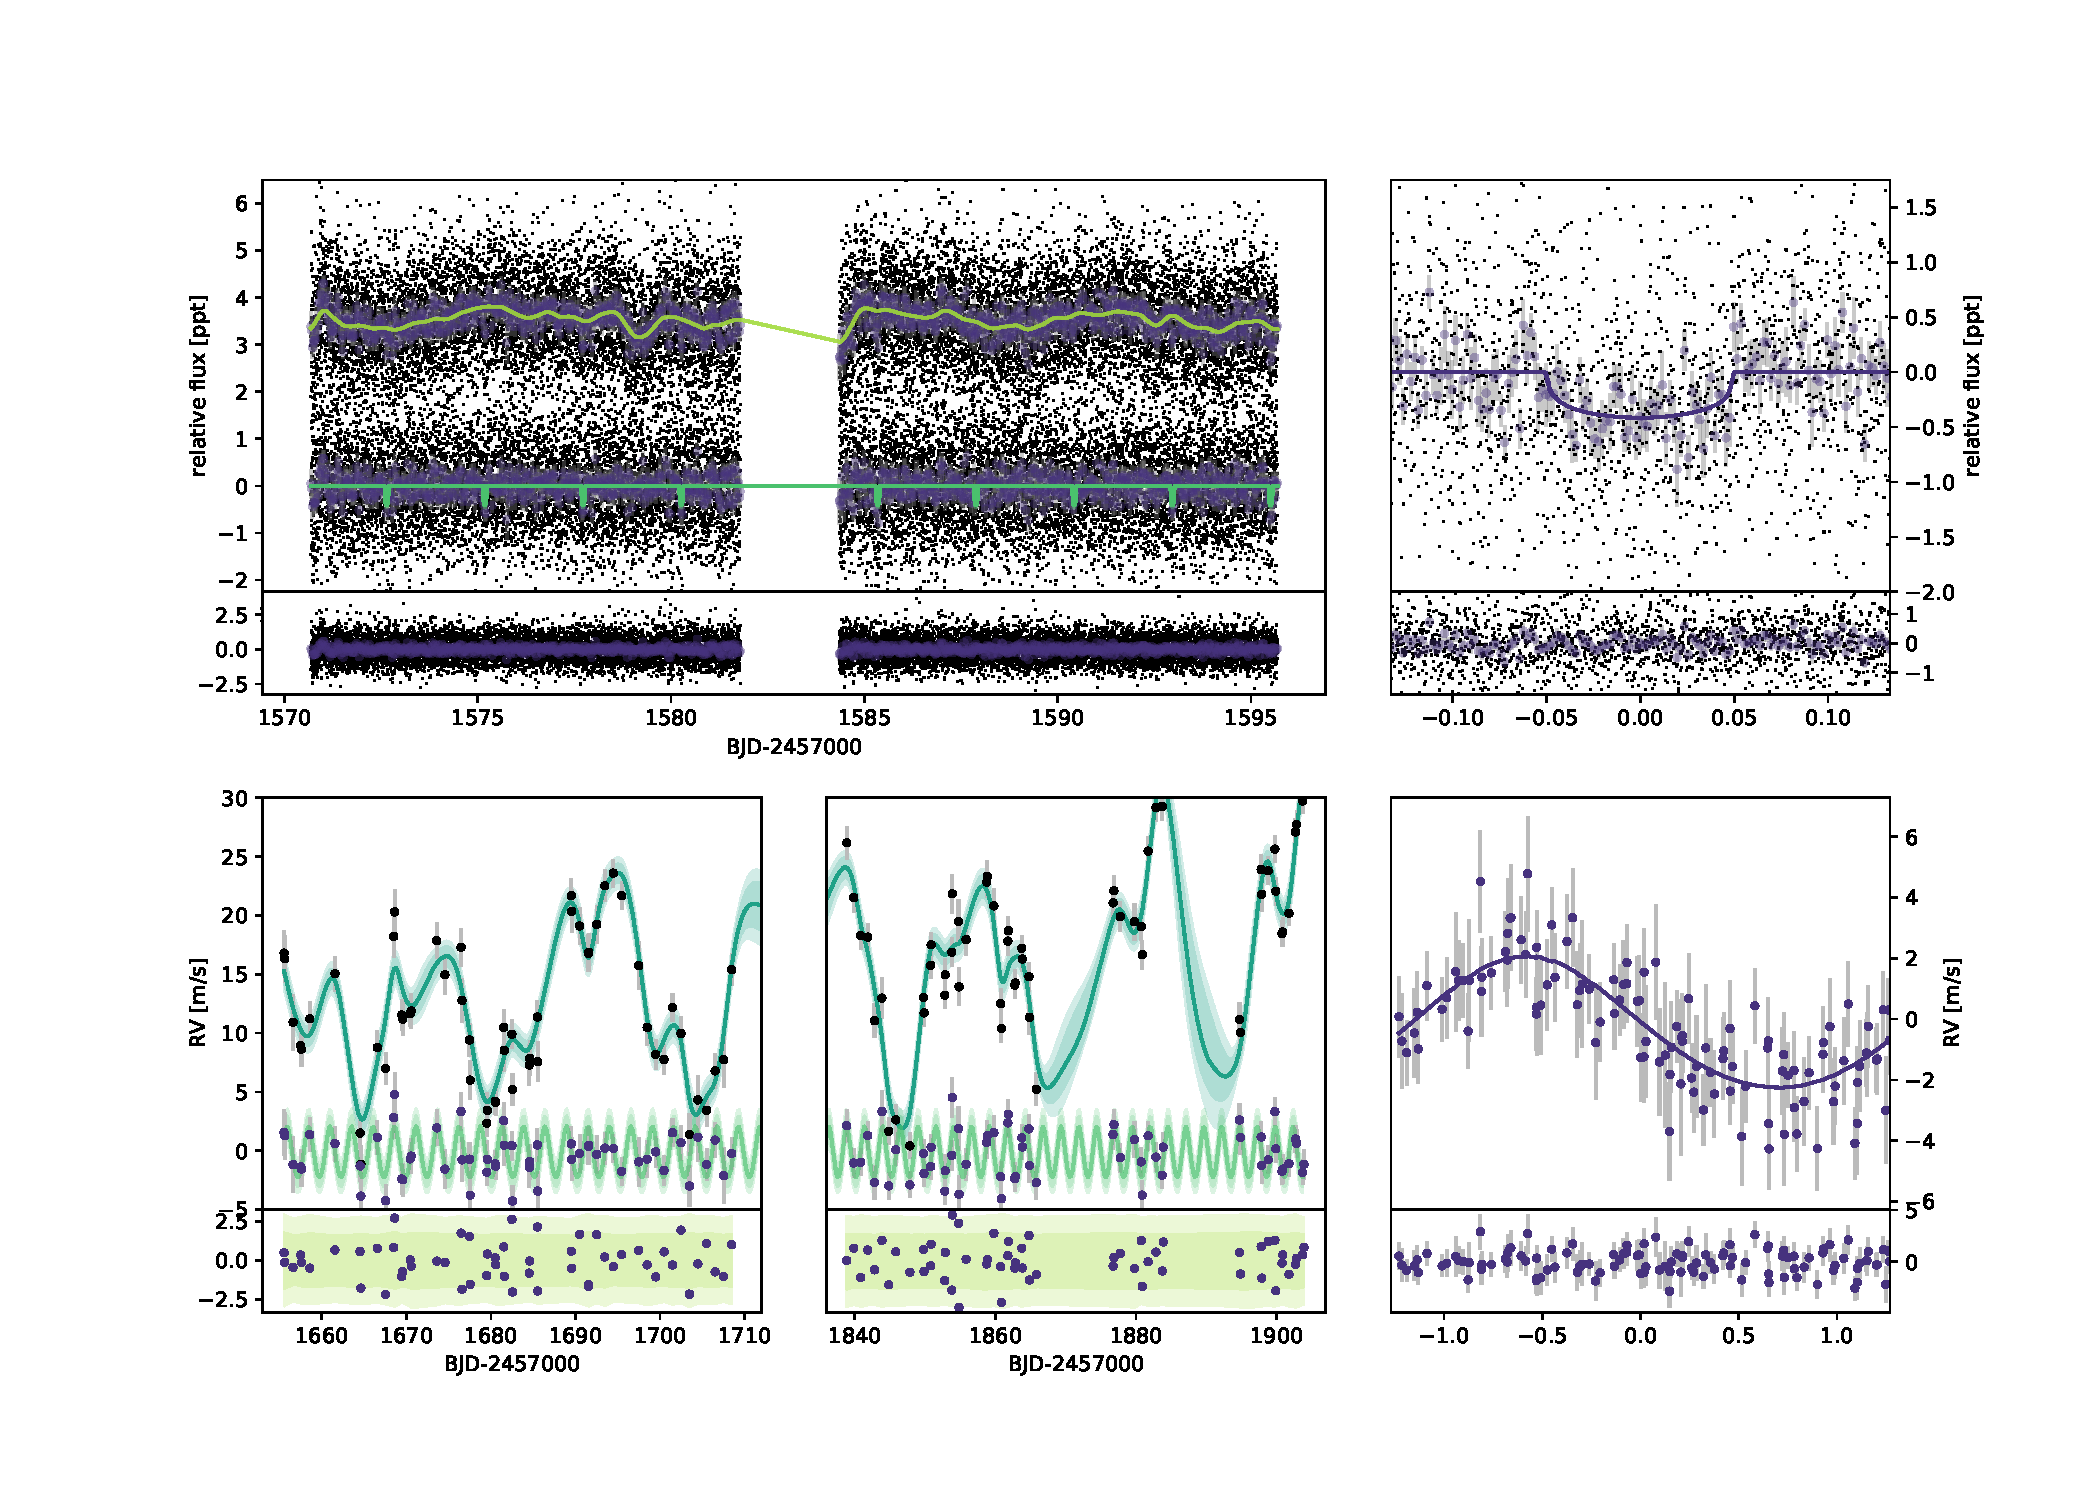
\includegraphics[width=\paperwidth]{Combined_Model_plots_2xGP_smooth}
% }
% \caption{Photometric \& RV time series.
% Detrended \tess Lightcurve both with and without best-fit Gaussian Process; transit model lightcurve residuals after subtraction of GP and transit model (centre left);
% Phase-folded lightcurve centred on transit with best-fit model (upper right); Phase-folded model residuals (centre right);
% Detrended \harps RVs both with and without S-index-trained Gaussian Process model (lower left); 
% RV residual time series after subtraction of GP and planet model (bottom left);
% Phase-folded RVs with best-fit RV model (lower right); Phase-folded RV residuals (bottom right).
% }
% \label{FullTransitFits0}
% \end{figure*}

\subsection{Discussion}


\begin{figure}
	% To include a figure from a file named example.*
	% Allowable file formats are eps or ps if compiling using latex
	% or pdf, png, jpg if compiling using pdflatex
	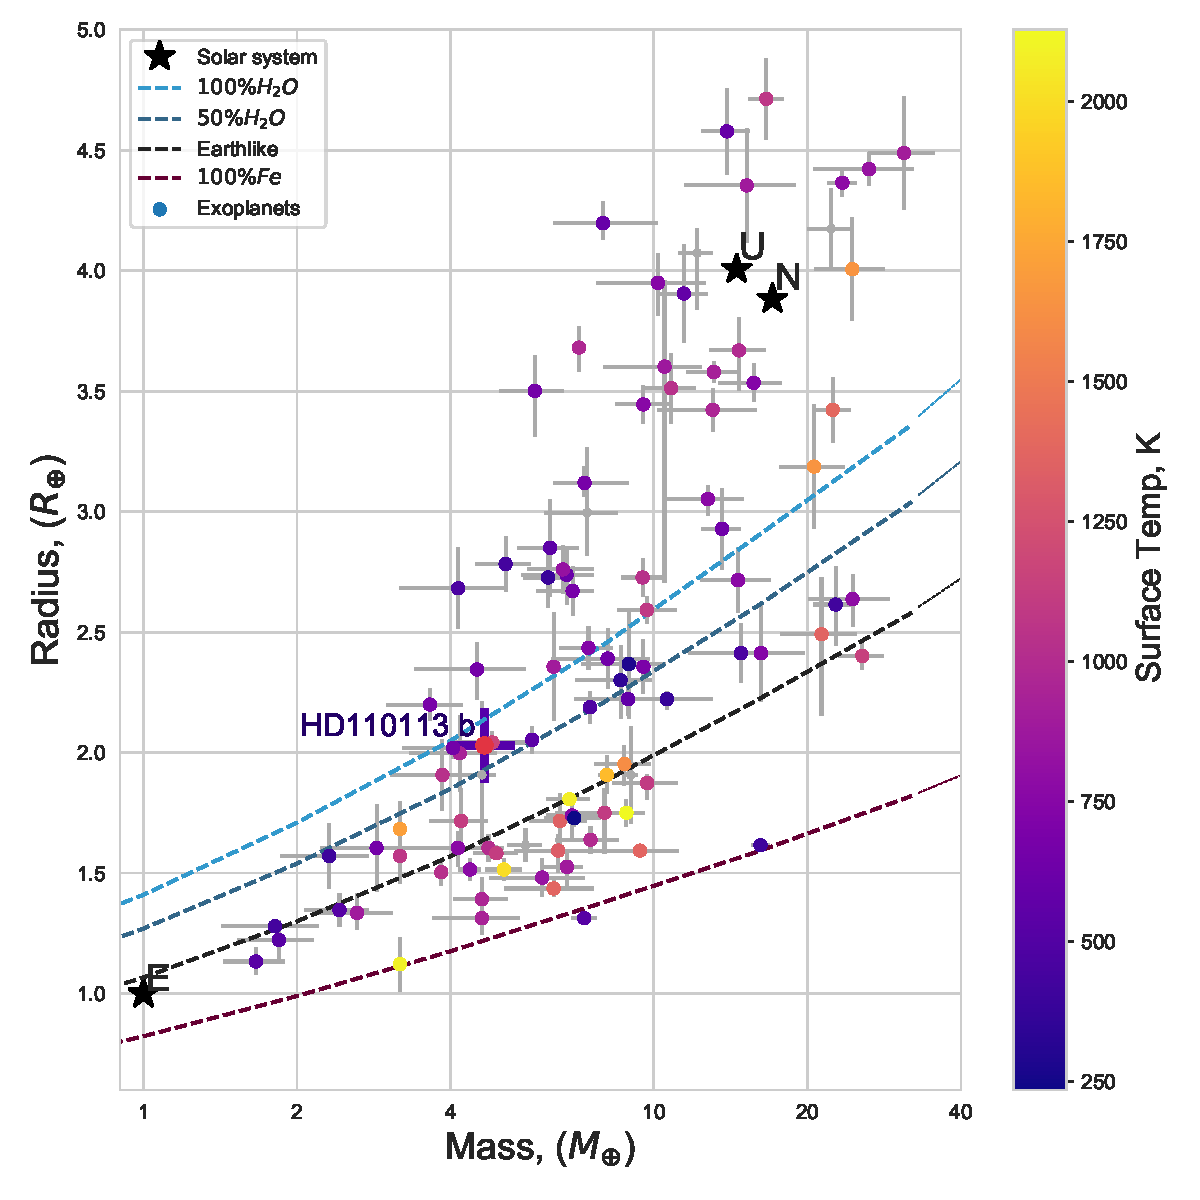
\includegraphics[width=\columnwidth]{MR_Diagram_sm}
    \caption{A Mass-Radius diagram for small planets with masses and radii constrained to better than SNR=4, with data from the NASA exoplanet archive \citep{akeson2013nasa}. Colour coding shows the surface temperature of each planet (assuming an albedo of 0.2). Solar System planets are marked with stars.}
    \label{fig:example_figure}
\end{figure}

% Example table
\begin{table}
	\centering
	\caption{This is an example table. Captions appear above each table.
	Remember to define the quantities, symbols and units used.}
	\label{tab:example_table}
	\begin{tabular}{lccr} % four columns, alignment for each
		\hline
		A & B & C & D\\
		\hline
		1 & 2 & 3 & 4\\
		2 & 4 & 6 & 8\\
		3 & 5 & 7 & 9\\
		\hline
	\end{tabular}
\end{table}

\onecolumn
\centering
\begin{table*}
\caption{List of free parameters used in the \texttt{exoplanet} combined analysis of the \tess{} light curve and \harps{} radial velocities with their associated prior and posterior distributions.}
\label{tab:plantparlong}
\begin{center}
\begin{tabular}{lcc}
\hline
\hline
Parameter & Prior & Posterior\\
\hline
\hline
\multicolumn{3}{l}{\it Stellar parameters}\\
Stellar surface temperature, \teff{} [K] &  $\mathcal{N}(5732.0,16.0)$  &   $ 5731.0 \pm 16.0 $ \\
Stellar surface gravity, \logg{} [cgs] &  $\mathcal{N}(4.46,0.02)$  &   $ 4.46 \pm 0.02 $ \\
Stellar Metallicity \feh{} &  $\mathcal{N}(0.14,0.02)$  &   $ 0.14 \pm 0.02 $ \\
Stellar Mass, $M_s$ [$M_{\odot}$] &  $\mathcal{N}(0.997,0.0095)$  &   $ 0.9968 \pm 0.0096 $ \\
Stellar Radius, $R_s$ [$R_{\odot}$] &  $\mathcal{N}(1.035,0.026)$  &   $ 1.033^{+0.025}_{-0.026} $ \\
\hline
\multicolumn{3}{l}{\it Orbital parameters}\\
Transit Epoch, $t_0$ [BJD-2457000] b &  $\mathcal{N}(1570.101893,0.1)$  &   $ 1570.1009 \pm 0.0042 $ \\
Transit Epoch, $t_0$ [BJD-2457000] c &  $\mathcal{N}(1798.1334,13.5)$  &   $ 1798.11^{+0.19}_{-0.26} $ \\
Orbital Period, $P$ [d] b &  $\mathcal{N}_{\mathcal{U}}(2.540455,0.000708,2.35,2.6)$  &   $ 2.54074 \pm 0.00043 $ \\
Orbital Period, $P$ [d] c &  $\mathcal{N}_{\mathcal{U}}(6.7285,0.00541,6.65,6.8)$  &   $ 6.7329 \pm 0.0048 $ \\
Orbital Eccentricity b &  $\beta(0.867;3.03)$  &   $ 0.092^{+0.079}_{-0.067} $ \\
Orbital Eccentricity c &  $\beta(0.867;3.03)$  &   $ 0.063^{+0.094}_{-0.048} $ \\
Argument of periasteron, $\Omega$ b &  $\mathcal{U}(-\pi,\pi)^{\tnote{a}}$  &   $ -0.2 \pm 1.0 $ \\
Argument of periasteron, $\Omega$ c &  $\mathcal{U}(-\pi,\pi)^{\tnote{a}}$  &   $ -0.1 \pm 1.2 $ \\
\hline
\multicolumn{3}{l}{\it Photometric parameters}\\
log radius ratio [$\log{R_p/R_s}$] b &  $\mathcal{U}(-4.6,-2.3)$  &   $ -3.939 \pm 0.07 $ \\
log radius ratio [$\log{R_p/R_s}$] c &  $\mathcal{U}(-11.51,-2.3)$  &   $ -7.7 \pm 2.6 $ \\
Transit Impact Parameter b & $\mathcal{U}(0,1+R_p/R_s)^{\tnote{b}}$  &   $ 0.43 \pm 0.21 $ \\
Transit Impact Parameter c & $\mathcal{U}(0,1+R_p/R_s)^{\tnote{b}}$  &   $ 0.5 \pm 0.34 $ \\
Quadratic Limb Darkening $a_{\rm LD}$ &  $\mathcal{N}_{\mathcal{U}}(0.367,0.1,0.0,1.0)$  &   $ 0.371 \pm 0.1 $ \\
Quadratic Limb Darkening $b_{\rm LD}$ &  $\mathcal{N}_{\mathcal{U}}(0.21,0.1,0.0,1.0)$  &   $ 0.216^{+0.098}_{-0.093} $ \\
Photometric jitter [$\log{\rm ppt}$] &  $\mathcal{N}(-0.158,3.0)$  &   $ -4.8^{+1.0}_{-1.6} $ \\
Photometric GP power & $\mathcal{I}{0.014,0.006}^{\tnote{c}}$  &   $ 0.0118^{+0.0034}_{-0.0025} $ \\
Photometric GP frequency [$d^{-1}$] & $\mathcal{I}{3.525,0.651}^{\tnote{c}}$  &   $ 3.61 \pm 0.42 $ \\
Photometric GP mean [ppt] & $\mathcal{I}{0.008,0.036}^{\tnote{c}}$  &   $ 0.009^{+0.032}_{-0.035} $ \\
\hline
\multicolumn{3}{l}{\harps{} parameters}\\
log RV semi-amplitude b &  $\mathcal{N}(0.693,10.0)$  &   $ 0.77 \pm 0.13 $ \\
log RV semi-amplitude c &  $\mathcal{N}(0.693,10.0)$  &   $ 1.27 \pm 0.11 $ \\
RV trend - intercept at BJD=2458779.717 [\ms{}] &  $\mathcal{N}(0.0,0.1)$  &   $ 0.0126^{+0.0056}_{-0.005} $ \\
RV trend - gradient [\ms{}$d^{-1}$] &  $\mathcal{N}(0.0,1.0)$  &   $ -0.02 \pm 0.96 $ \\
\harps{} log jitter RV [\ms{}] &  $\mathcal{N}(-0.5,2.0)$  &   $ -0.3 \pm 0.9 $ \\
\harps{} log jitter S index &  $\mathcal{N}(-0.5,2.0)$  &   $ -12.28 \pm 0.41 $ \\
\harps{} log jitter FWHM [\ms{}] &  $\mathcal{N}(-0.5,2.0)$  &   $ -1.3^{+1.5}_{-1.7} $ \\
\harps{} mean RV [\ms{}] &  $\mathcal{N}(0.0,7.3303)$  &   $ -0.4 \pm 2.2 $ \\
\harps{} mean S index &  $\mathcal{N}(0.0,0.0094)$  &   $ -0.0006 \pm 0.0013 $ \\
\harps{} mean FWHM [\ms{}] &  $\mathcal{N}(7287.75,7.4997)$  &   $ 7286.8 \pm 1.2 $ \\
\harps{} GP log amplitude RV [\ms{}] &  $\mathcal{N}(-0.621,8.0)$  &   $ 3.68 \pm 0.4 $ \\
\harps{} GP log amplitude S index &  $\mathcal{N}(-13.937,8.0)$  &   $ -9.66 \pm 0.4 $ \\
\harps{} GP log amplitude FWHM [\ms{}] &  $\mathcal{N}(-0.575,8.0)$  &   $ 2.92^{+0.63}_{-0.84} $ \\
\harps{} GP decay log timescale, $\log{\tau}/\log{d}$ &  $\mathcal{U}(-0.061,5.0)$  &   $ 2.4 \pm 1.7 $ \\
\harps{} GP log rotation period, $\log{P_{\rm rot}}/\log{d}$ &  $\mathcal{N}_{\mathcal{U}}(3.02,0.4,1.1,4.38)$  &   $ 3.049^{+0.076}_{-0.046} $ \\
\harps{} GP log quality &  $\mathcal{N}(1.0,10.0)$  &   $ -0.7^{+1.6}_{-3.3} $ \\
\harps{} GP log quality differential &  $\mathcal{N}(2.0,10.0)$  &   $ 0.5^{+1.3}_{-6.3} $ \\
$P_{\rm rot}$ - $P_{\rm rot}/2$ mix factor &  $\mathcal{U}(0,1)$  &   $ 0.05^{+0.11}_{-0.04} $ \\
\hline
\hline
\end{tabular}
\tablefoot{$\mathcal{N}(\mu;\sigma^{2})$ is a normal distribution with mean $\mu$ and width $\sigma^{2}$, $\mathcal{U}(a;b)$ is a uniform distribution between $a$ and $b$, $\mathcal{N}_{\mathcal{U}}(\mu;\sigma^{2},a,b)$ is a normal distribution with mean $\mu$ and width $\sigma^{2}$ multiplied with a uniform distribution between $a$ and $b$, $\beta(a;b)$ is a Beta distribution with parameters $a$ and $b$, and $\mathcal{I}(\mu;\sigma^2)$ is a distribution directly interpolated from the output of a pre-trained distribution with mean $\mu$ and standard deviation $\sigma^2$. 
Posterior values and uncertainties represent the median and $1\sigma$ error boundaries.
All other values (e.g. presented in Table \ref{tab:plantparshort}) are directly determined from these fitted quantities.
\tnote{a} Described in \citet{kipping2013parametrizing}. 
\tnote{a} Reparameterised in \texttt{exoplanet} to avoid discontinuities at $\pm\pi$.
\tnote{c} \texttt{exoplanet} reparameterization of \citet{espinoza2018efficient}.
\tnote{e} \texttt{PyMc3} Interpolation function of pre-trained GP.} %citation to Kipping (2013)
\end{center}
\label{AllPriors}
\end{table*}%
\twocolumn

\section{Conclusions}

The last numbered section should briefly summarise what has been done, and describe
the final conclusions which the authors draw from their work.

\section*{Acknowledgements}
This research made use of \textsf{exoplanet} \citep{exoplanet} and its
dependencies \citep{exoplanet:agol19, exoplanet:astropy13, exoplanet:astropy18,
exoplanet:exoplanet, exoplanet:foremanmackey17, exoplanet:foremanmackey18,
exoplanet:luger18, exoplanet:pymc3, exoplanet:theano}.


%%%%%%%%%%%%%%%%%%%%%%%%%%%%%%%%%%%%%%%%%%%%%%%%%%

%%%%%%%%%%%%%%%%%%%% REFERENCES %%%%%%%%%%%%%%%%%%

% The best way to enter references is to use BibTeX:

\bibliographystyle{mnras}
\bibliography{example} % if your bibtex file is called example.bib


% Alternatively you could enter them by hand, like this:
% This method is tedious and prone to error if you have lots of references
%\begin{thebibliography}{99}
%\bibitem[\protect\citeauthoryear{Author}{2012}]{Author2012}
%Author A.~N., 2013, Journal of Improbable Astronomy, 1, 1
%\bibitem[\protect\citeauthoryear{Others}{2013}]{Others2013}
%Others S., 2012, Journal of Interesting Stuff, 17, 198
%\end{thebibliography}

%%%%%%%%%%%%%%%%%%%%%%%%%%%%%%%%%%%%%%%%%%%%%%%%%%

%%%%%%%%%%%%%%%%% APPENDICES %%%%%%%%%%%%%%%%%%%%%

\appendix

\section{Some extra material}

If you want to present additional material which would interrupt the flow of the main paper,
it can be placed in an Appendix which appears after the list of references.

%%%%%%%%%%%%%%%%%%%%%%%%%%%%%%%%%%%%%%%%%%%%%%%%%%


% Don't change these lines
\bsp	% typesetting comment
\label{lastpage}
\end{document}

% End of mnras_template.tex